%% ----------------------------------------------------------------
%% Progress.tex
%% ---------------------------------------------------------------- 
\documentclass{ecsprogress}   % Use the progress Style
\graphicspath{{/Figures/}} 
\newcommand{\code}[1]{\texttt{#1}}
\usepackage[backend=biber, style=authoryear]{biblatex}  % Location of your graphics files
\addbibresource{Bibliography.bib}
%\usepackage{natbib}         % Use Natbib style for the refs.
\usepackage{tabu}
\usepackage{float}
\hypersetup{colorlinks=true}   % Set to false for black/white printing
%
\definecolor{purple}{rgb}{0.65, 0.12, 0.82}
\lstset{
	breakatwhitespace=true,
	breaklines=true,
	keywordstyle=\color{blue}\bfseries,
	identifierstyle=\color{black},
	commentstyle=\color{purple}\itshape,
	stringstyle=\color{red},
	float=here
}

\lstdefinelanguage{javascript}{
	keywords={break, case, catch, continue, debugger, default, delete, do, else, false, finally, for, function, if, in, instanceof, new, null, return, switch, this, throw, true, try, typeof, var, void, while, with},
	morecomment=[l]{//},
	morecomment=[s]{/*}{*/},
	morestring=[b]',
	morestring=[b]",
	ndkeywords={class, export, boolean, throw, implements, import, this},
	sensitive=true
}            % Include your abbreviations
%% ----------------------------------------------------------------
\begin{document}
\frontmatter
\title      {An Investigation into \dots}
\authors    {\texorpdfstring
             {\href{mailto:stp1g15@ecs.soton.ac.uk}{Steffan T. Padel}}
             {Steffan T. Padel}
            }
\addresses  {\groupname\\\deptname\\\univname}
\date       {\today}
\subject    {}
\keywords   {}
\supervisor {Prof. Adam Prugel-Bennett}
\examiner   {Prof. Lie-Liang Yang}
\maketitle
\begin{abstract}
This work is all about \dots
\end{abstract}
\tableofcontents
\listoffigures
\listoftables
\lstlistoflistings
\listofsymbols{ll}{$w$ & The weight vector}
\acknowledgements{Thanks to no one.}
\dedicatory{To \dots}
\mainmatter
%% ----------------------------------------------------------------
\chapter{Introduction}

\section{Problem}
While learning a second language, many learners encounter problems while trying to find and read texts written in the language they are learning. Modern technology has helped with this to some regard, with development of glosses, which are digital tools that provide prompts for vocabulary words. These prompts can be translations of the words, definitions in the source language, audio visual materials or any combination of the above. 

The problem most glosses developed today have is that they are specifically tailored for the text they are being used on. The words that can be examined are pre-selected, the gloss content is pre-written and the text has been pre-selected. This still leaves multiple problems for the user: They could not find the text interesting, they could already know the words in the gloss or they might find the text too easy. 

\section{Solution and Goals}

The solution to this problem was, perhaps unsurprisingly, to develop a prototype application. This application should be able to:

\begin{itemize}
	\item Allow the user to a select a category of articles that they find interesting.
	
	\item Find and pull articles in that category from a variety of news sources.
	
	\item Rate the articles based on their perceived difficulty for the user.
	
	\item Allow the user to activate a gloss on any and all words in the article. 
\end{itemize}

To make sure as many platforms are supported as easily as possible, the application will run in a web browser and be hosted remotely. The initial prototype of the application will support German in order to minimise the number of variable that need to be taken into account and because German is a language the developer can speak, allowing for easier development of the application.

Once developed, this  prototype application will then be user tested by a number of German learners of varying experience levels. They will provide feedback on their experiences using the application, which will then be examine and used to formulate the idea of a release build. 
\chapter{Background Reading}

Reading for the project can be divided into reading about the gloss aspect of the application, and then reading about a difficulty rating system. Each of these parts of the reading happened independently, as their subject matter are largely unrelated.


\section{Glosses}

The research done into glosses is divided into to parts, the first being research into whether or not glosses are effective, the second part was about the various designs of glosses, trying to discover which ones were the most effective.

\subsection{Effectiveness of Electronic Glosses}

\textcite{abraham2008} finds that, overall, that learners with access to an electronic gloss will perform better than learners without access, in both skills of reading comprehension and vocabulary retention, particularly on intermediate learners. They note that the small sample size of studies analysed should mean that their study is not seen as conclusive evidence, however suggestive evidence is enough to establish that development of this project should continue.

Another caveat that should also be added that most of the studies analysed in \textcite{abraham2008} are of tailor-made glosses designed for a specific text, as such the research findings of these studies and the meta-study may not be fully applicable to this project.


\subsection{Design Methods of Electronic Glosses}

\textcite{roby1999} identifies three main parts of a gloss' design, its presentation, its taxonomy and its density. However, as density, which is the amount of content in the gloss, is something determined by the user, background reading into design was limited to presentation and taxonomy. 

\subsubsection{Gloss Presentation}

Gloss presentations is how the gloss is presented relative to the text. 

\textcite{chen2016} identifies the three most researched gloss presentations as: in-text, marginal and pop up.  \textcite{abuseileek2008} finds that out of these three the marginal presentation category performs the best in both vocabulary retention and reading comprehension, while \textcite{marefat2016} finds that pop-ups are more effective than marginal for reading comprehension. As \textcite{chen2016} says, there has not been sufficient research into gloss location for valid conclusions to be drawn. 

\subsubsection{Gloss Taxonomy}

Gloss taxonomy is the content of the gloss.

\textcite{gettys2001} finds that dictionary style translations perform better than sentence level translations, suggesting that it would be better to translate the dictionary form of the word, providing information about how the word changed from its dictionary form to its current form in the article. 

There is a large body of research that suggests that providing multimedia glosses is more effective than providing text only ones. \autocite{yoshii2006, kost1999}. This is harder to implement  as it would the application to have a better understanding of the word's context to provided an accurate image of the word. 


\section{Article Difficulty Rating}

The reading for this section of the application was harder to find, little has been written about the discovery and difficulty rating of texts for second language learners in general, or German learners in specific. 

The easiest method of calculating the difficulty of an article seems to be a mathematical expression of it's readability, called a readability index. Perhaps the most famous of these being the Flesch Reading Ease (FRE) formula \autocite{flesch1948}. This formula is for America English, however similar formulae have been developed for German, two of these are highlighted below.

The first formula for German is an adaptation of the FRE formula as proposed in \textcite{amstad1978}, this relies on much the same model as the original FRE formula, however takes into account the longer average word length in the German language, this formula is show in figure \ref{fig:fre} where  ASL is the average sentence length and ASW is the average syllables per word. This formula maps the readability of the text onto a range of 0 to 100, with 0 being easy and 100 being hard. 

\begin{figure}[H]
	\caption[Flesch Reading Ease Formula]{Formula for the German adaptation of the Flesch reading ease formula, a method of calculating the readability of a German language text}
	\label{fig:fre}
	\begin{center}
		\begin{math}
		FRE = 180 - ASL - 58.5 \times ASW
		\end{math}
	\end{center}
\end{figure}

The other readability index for German is the  Wiener Sachtextformel (WSTF) as proposed in \textcite{bamberger1984}, on version of this is as shown in figure \ref{fig:wst}. Where MS is the percentage of words with three or syllables, SL is the average sentence length, IW is the percentage of words with six or more characters and ES is the percentage of monosyllabic words. This formula maps the difficulty rating onto a range of 4 to 15, with the lower numbers being easier. This is done to reflect the German school year that is believed to be appropriate for that level of text.

\begin{figure}
	\caption[Erste Wiener Sachtextformel Formula]{The Erste Wiener Sachtextformel formula, one method of calculating the readability of German language texts. }
	\label{fig:wst}
	\begin{center}
		\begin{math}
		WSTF = 0.1935 \times MS + 0.1672 \times SL + 0.1297 \times IW - 0.0327 \times ES - 0.875
		\end{math}
	\end{center}
\end{figure}

The two formulas are commonly used together when assessing the readability of texts, being used in a variety of studies, such as \textcite{rottensteiner2010} which uses them both to assess the readability of newly published textbooks. This publication also notes that these formulae only measure the linguistic complexity of the article, ignoring other factors, such as presentation, that influence how easy the article is to read. 

In addition to the formulae listed above there are methods of determining a readability ranking through the use of machine learning. \textcite{hancke2012} which attempts to build a readability classification system from a corpus of articles. This paper looks a lot more in depth at a lot of features of the text. However, this model only performed 7.5\% better than the computational scores calculated from the traditional formula. Given the time constraints and the already complex nature of the project, it would not be worth the effort to implement such a model, as the tradition formulae such as WSTF and FRE perform well enough for the purposes of this project. 
\chapter{Proposed Design \& Development}
\section{Design}
The project will be split into three views, the first, which will be similar to the wireframe in figure \ref{fig:view1} is a selection screen with a text area, where the user can select tags to search by inputting them.

\begin{figure}
	\caption[Screenshot of the Category Selection View]{Screenshot of the category selection view, where the user inputs the category of article they want to read, as well as their experience level.}
	\label{fig:view1}
	\begin{center}
	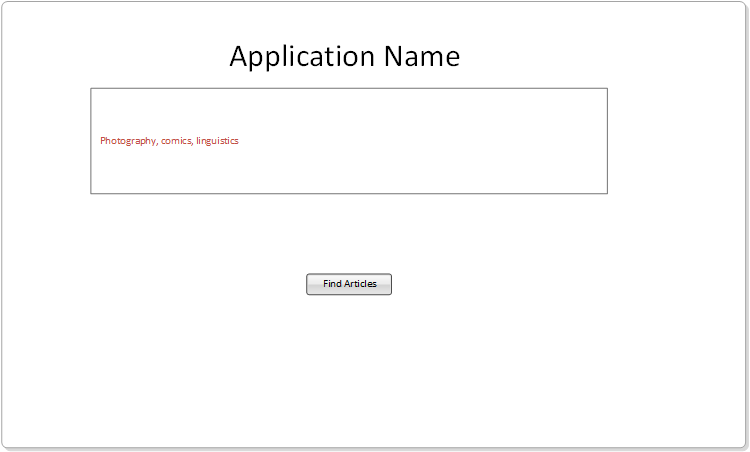
\includegraphics[width=\textwidth]{Graphics/View1}
	\end{center}
\end{figure}

Once the user inputs their preferred categories, the application takes those categories and finds relevant L2 articles by looking at articles on various sites, it then takes those articles and displays the title of each article, similar to view shown in figure \ref{fig:view2}

\begin{figure}
	\caption[Screenshot of the Article Selection View]{An example of the article selection view, here the user is shown a list of articles in their selected category as well as the difficulty rating for each article. They then go on to select an article from the list.}
	\label{fig:view2}
	\begin{center}
	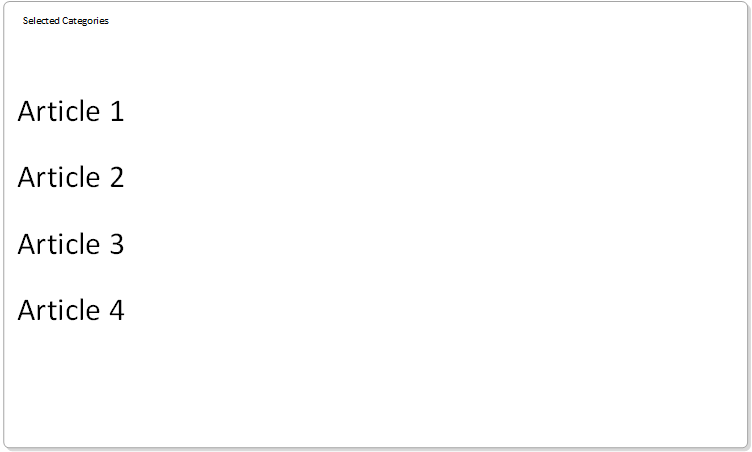
\includegraphics[width=\textwidth]{Graphics/View2}
\end{center}
\end{figure}

From the view shown in figure \ref{fig:view2} the user can select an article, once they do so, the application will download and parse the article, displaying it to the user, similar to the view in figure \ref{fig:view3}.

\begin{figure}
	\caption[Screenshot of the Article Reading View]{The article reading view, where the user can read the contents of their selected article. To the left of the article content is a button taking them back to article selection view and to the right is the gloss column, which contains a prompt telling the user click on articles. }
	\label{fig:view3}
	\begin{center}
	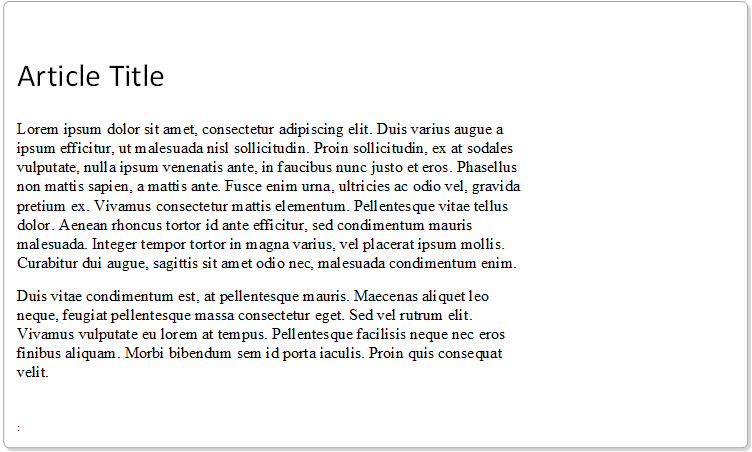
\includegraphics[width=0.7\textwidth]{Graphics/View3}
\end{center}
\end{figure}

from figure \ref{fig:view3} the user can select a word in the article, this action will send a request to the server for a gloss. The server will then look up translations of the word, along with grammatical information for the word, it will then serve the content, properly formatted, to the user, in a marginal gloss looking similar to the view in figure \ref{fig:view4}.

\begin{figure}
	\caption[Screenshot of the Article Reading View with Gloss]{Another screenshot of the article reading view, this time with a gloss entry in the margin.}
	\label{fig:view4}
	\begin{center}
	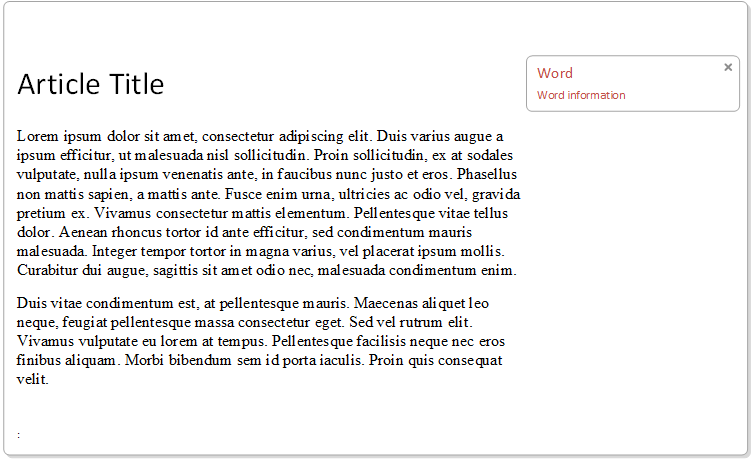
\includegraphics[width=\textwidth]{Graphics/View4}
\end{center}
\end{figure}

A marginal gloss in with multiple L1 translations and grammatical information as marginal glosses are effective \cite{abuseileek2008} and relatively easy to develop for. Multiple translations are being used to prevent the occurrence of an incorrect translation. 

The whole systems process is illustrated in figure \ref{fig:sf}.
	
\begin{figure}
	\caption{Wireframe Mockup of the Category Input View}
	\label{fig:sf}
	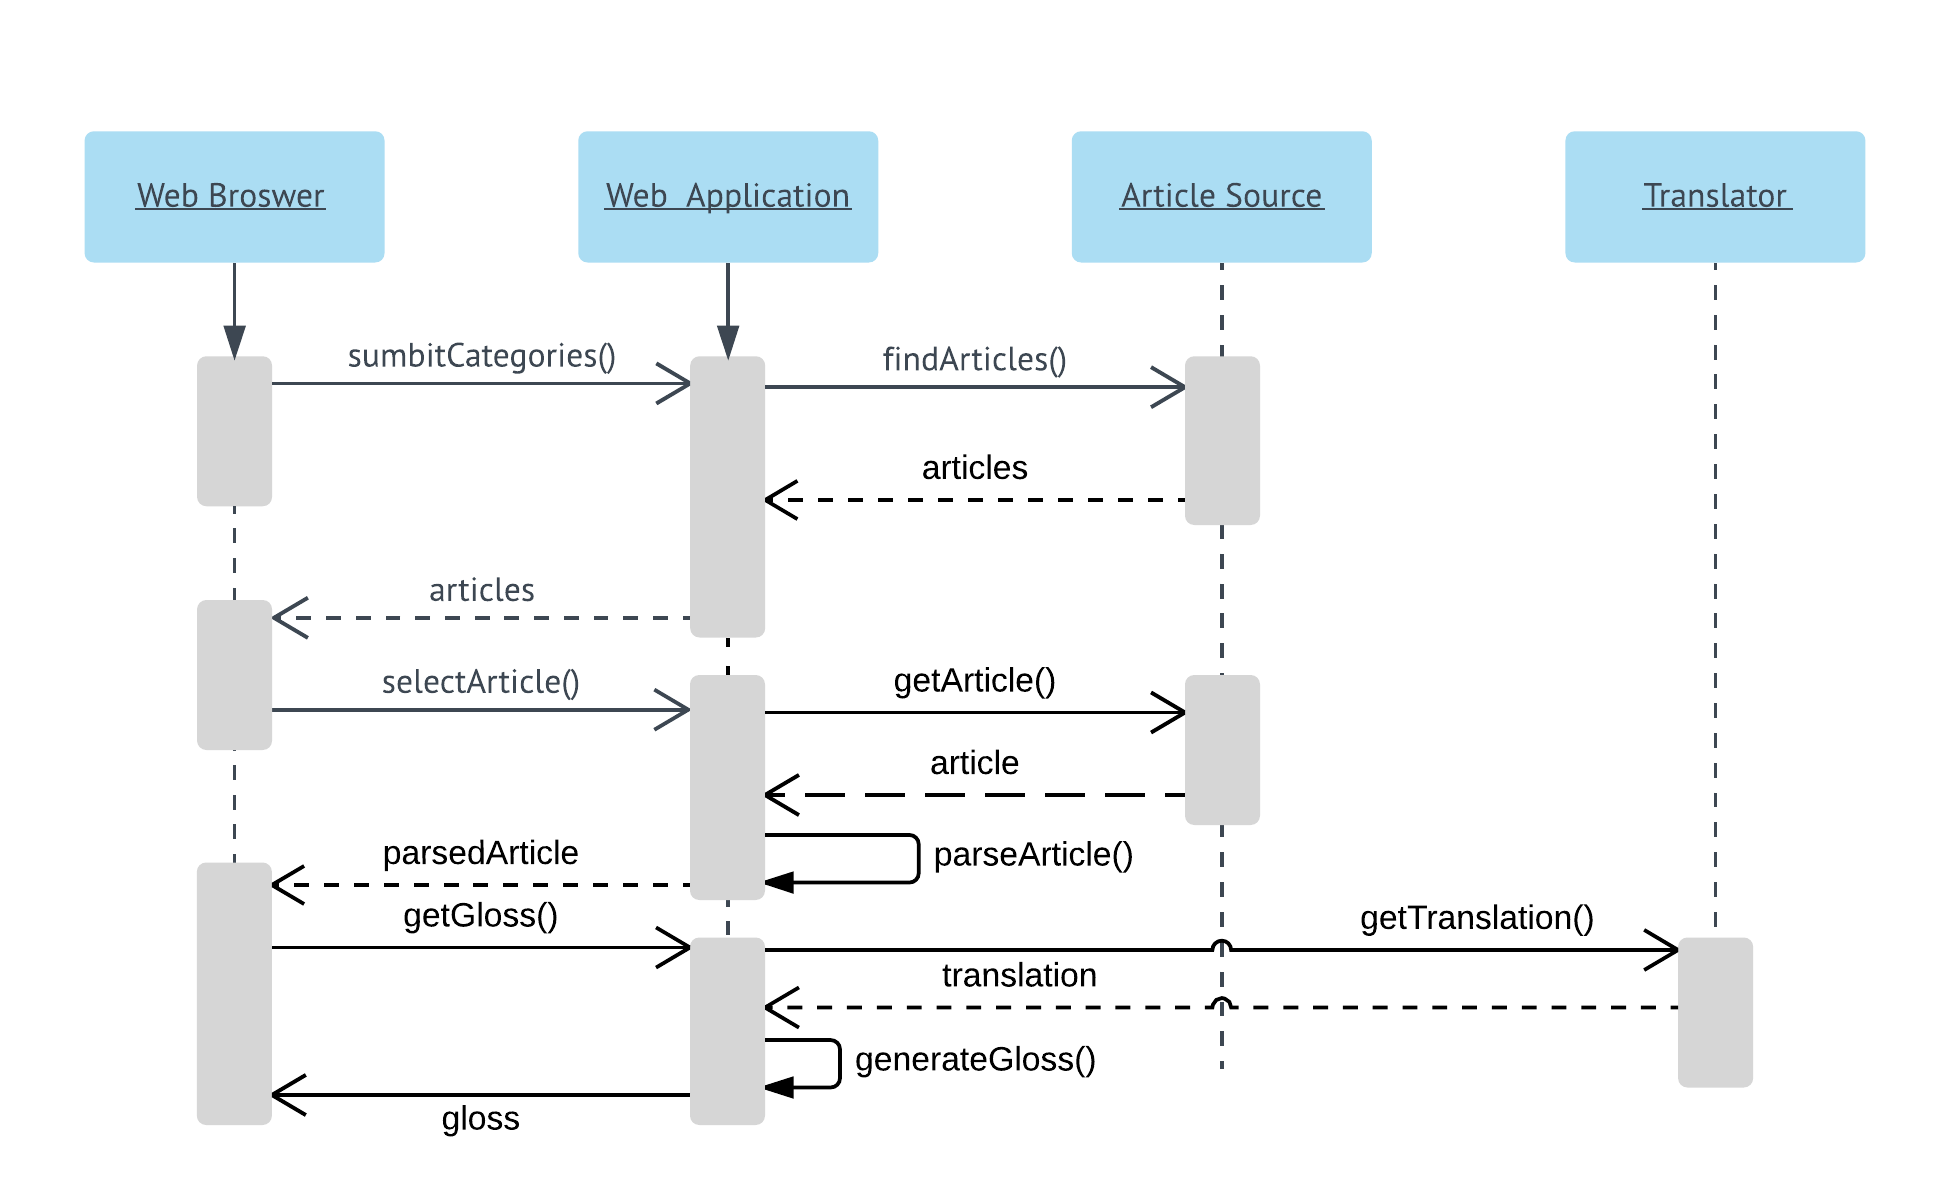
\includegraphics[width=\textwidth]{Graphics/SystemsFlow}
\end{figure}

\section{Development}

The plan is to develop the application using agile development structures using five sprints. Agile development was chosen because it allows for feedback to received on the project at weekly supervisor meetings, it also means that the development can be adjusted based on new ideas presented during the feedback session.

The five Sprints and their aims as as follows:
\begin{enumerate}
	\item \textbf{Translation Lookup}
	
	The aim of this sprint is to establish a valid method to retrieve single word translation and grammatical data.
	
	\item \textbf{Article Parsing \& Presentation}
	
	The aim of this sprint is develop a method for the parsing of articles and then to present them through a web browser
	
	\item \textbf{AJAX}
	
	The aim of this sprint is to develop the javscript code that will allow the gloss to display entries.
	
	\item \textbf{Recommender System}
	
	The aim of this sprint it to develop the recommender system that will suggest articles to the user. 
	
	\item \textbf{Advance Parsing}
	
	The aim of this sprint is to allow for advance parsing, such as parts of speech or the breaking up of German compound words into their component parts.
\end{enumerate}

These sprints were chosen as each of them represents a core development of a feature in the project. The order was chosen as it allows the project to reach minimum viable status as soon as possible (sprint 3). While leaving the most optional sprint until last.  

\section{Testing}
Preliminary testing will be done during and at the end of each sprint, this will allow the developer to test each part of the application, seeing if it works. Then the application as a whole will be tested. 

Once the five sprints have been completed, the application will have to be user-test to make sure it performs effectively. Users will test the application by using it, then answering a questionnaire about the application and their experiences using it. 

Splitting the testing into two main parts like this means that the testing of each indivual part will be completed in time for user testing, so the users will only ever been testing the complete application. Not performing user testing until the end of the project will mean that only one ethics approval will have to be submitted. 
\chapter{Work Done So Far}
Sprints One, Two and Three have been completed as of the time of writing.

\section{Sprint One - Dictionary Lookup}
The sprint began by looking into technologies to translate the word being clicked on. Possibilities considered were online translation services such as \textcite{googletranslate} and \textcite{bingtranslate}, raw datasets such as the \textcite{dictCC} and Dictionary APIs such as the \textcite{oxford} and the \textcite{collins}. 

The technology that would be used in the project would have to:
\begin{itemize}
	\item Be able to translate single words from to English
	\item Provide Lexical information of those words
	\item Be allowed for the content to be hosted and provided through a web interface
	\item Be available for less than \pounds150 total
\end{itemize}

The five technologies cited above were checked against these criteria and the results are show in Table \ref{tbl:comp}

\begin{table}
\centering
\caption[Comparison of Translation Software]{Comparison of various translation solutions to see whether or not they fulfil the criteria of the application. }
\label{tbl:comp}
\begin{tabu} to \textwidth{|X[c]|X[c]|X[c]|X[c]|X[c]|}
\hline
\textbf{Product}        & \textbf{German to English Translations} & \textbf{Lexical Information} & \textbf{Allowed Online} & \textbf{Less Than \pounds150  (total)} \\ \hline
Google Cloud Translate  & Yes                                     & No                           & Yes                     & No                               \\ \hline
Microsoft Translator    & Yes                                     & No                           & Yes                     & No                               \\ \hline
Dict.cc Dataset         & Yes                                     & Yes                          & No                      & Yes                              \\ \hline
Oxford Dictionaries API & Yes                                     & Yes                          & Yes                     & Yes                              \\ \hline
Collins Dictionary API  & Yes                                     & Yes                          & Yes                     & No                               \\ \hline
\end{tabu}
\end{table}

As \textcite{oxford} was the only technology to clear all four criteria, the decision was made to used it for development of the application, however other technologies were used in testing the resulting code.

\textcite{oxford} is a REST API where two calls are required to get the desired information. The first, to the lemmatron, checks that the word is in the dictionary and provides a list of entries of unconjugated words, their lexical categories and grammar information. The second call is to lookup translations of this uncojugated word.

On the first call, the application takes the first entry provided by the response and extracts the root of the word along with the lexical category and the grammar of the conjugation. Then, on the second call, it compares lexical categories to ensure it's the correct word, before extracting English translations of the root. This information is then passed to a storage class.

Once this part of the application had been written, it was unit tested with a selection of random German words, the unconjugated word, translations and lexical information were compared to results provided by the other technologies and the developer's knowledge. The code passed testing as the results provided were accurate and contained the necessary grammatical information. 

The code for this sprint can be seen in listing \ref{app:dictcode}

\section{Sprint Two - Article Parsing \& Presentation}

A parsing library was used that returns the content of the article as a single string.  As each word would be clicked on individually in the application, a function was written that took this string an returned a two dimensional. The first dimension being paragraphs and the second one being alternating strings of words and punctuation so that each word was individually accessible. This array, was then written to a storage class, along with various bits of meta data that was either extracted by the parsing library or retrieved separately.  

The code for this part of sprint two can be seen in listing \ref{app:parsing}

The second part of this sprint was to enable for these parsed articles to be displayed. For this, a web application was written. This app displayed the parsed article on the left, with a margin on the right left for the gloss content. This view is shown in figure \ref{fig:article}. Each word extracted while parsing was wrapped in a span tag, allowing for easier identification by the AJAX.

The code for this part of the sprint can be seen in listings \ref{app:flask} (web  app) and \ref{app:article} (article display template)

The whole sprint was then tested by displaying some articles from the German website "Spiegel Online". The articles displayed nicely and the content of the text was correct, so the sprint passed the tests.

\section{Sprint Three - AJAX}

Sprint three was to connect the now displayed article with the dictionary api, allowing for the translations of a word to appear in the margin, once that word is clicked on. To do this, a function was assigned to the on-click listener of the span tag surrounding each word. When this function was called, a request would be sent to the server containing the word. The word is then be passed to the dictionary code written in sprint one, where the translations and lexical information would be retrieved from \textcite{oxford}. This information is then passed into a template and sent back to the webpage, where the new template is inserted into the margin on the right. 

CSS classes for the various lexical categories were defined to give each lexical category its own colour scheme, and the ability to remove entries was implemented by adding close button in the top right corner of the entry, with the appropriate function. 

The code was then tested using the same articles used in sprint two, making sure that the gloss entries were displayed as expected, and that they were for the right word and the content displayed in them was correct. 

The code for this sprint can be found in listings \ref{app:javascript} (javascript) and \ref{app:dictcss} (css classes)


\chapter{Work To Be Done}

Sprints four and five are still to be done before the final report, in addition to user testing and research into recommender systems.

\section{Sprint Four - Recommender Systems}

The recommender system of the application will suggest articles based on in-putted categories, recently published articles, and previous read articles. 

In order to understand how best to build a recommender system, reading will have to be done into which recommender systems are effective in finding relevant articles and what data these systems require. Once this reading has been done, the development of the systems to collect and store the required data will done, followed by the development of the recommender system itself.

Once the system has been built, it will be testing by inputting categories, and then seeing if the articles being returned are indeed relevant to those categories. 

\section{Sprint Five - Advanced Parsing }

The lookup method as of sprint three fails to successfully identify the types of words being used and also fails with longer compound words. The two parts of this sprint are to fix those two problems.

The first is to implement a parts of speech parser on the article, allowing the program to identify how the word is being used in the sentence, and find the dictionary entry with the correct lexical category or tense.

The second is that if a direct translation of a compound word is not in the dictionary, the application should attempt to break the compound word into its component parts and then provide a translation of each individual part. 

This sprint will then be tested by using the lookup tool to test words in less common situations and longer compound words.
\section{User Testing}

User testing of the application is the most vital thing to be done, but first it will require approval from the ethics committee. The plan is to request ethics approval during the first week of the winter holidays, which will hopefully result in approval by a week after the exams period. 

Once ethical clearance has been given, the application will be tested with various intermediate level German learners, They will be asked to use application to find articles of interest and then read these articles with the gloss. They will then be asked to fill out a survey, about whether or not they found the application improved their reading comprehension and vocabulary size, if they would continue to use the application. Whether or not they found the articles recommended interesting. 

The data from this survey will then be aggregated and analysed to see if the project was successful in its goals. 
\appendix
\chapter{Application Code}
\renewcommand{\SS}{\symbol{"1E9E}}

\lstset{breakatwhitespace=true, breaklines=true, inputencoding=utf8, literate={ä}{{\"a}}1 {ö}{{\"o}}1  {ü}{{\"u}}1 {ß}{{\ss}}1 {Ä}{{\"A}}1 {Ö}{{\"O}}1 {Ü}{{\"U}}1 {ẞ}{{\SS}}1}

\lstinputlisting[caption=third\_year\_project.py, title=third\_year\_project.py, label=app:flask ]{/home/nightwing/Documents/PycharmProjects/ThirdYearProject/third_year_project.py}

\lstinputlisting[caption=reader.py, title=reader.py, label=app:parsing]{/home/nightwing/Documents/PycharmProjects/ThirdYearProject/reader.py}

\lstinputlisting[caption=dictionary.py, label=app:dictcode, title=dictionary.py]{/home/nightwing/Documents/PycharmProjects/ThirdYearProject/dictionary.py}

\lstinputlisting[caption=templates/article.html, label=app:article, title=templates/article.html]{/home/nightwing/Documents/PycharmProjects/ThirdYearProject/templates/article.html}

\lstinputlisting[caption=templates/entry.html, label=app:entry, title=templates/entry.html]{/home/nightwing/Documents/PycharmProjects/ThirdYearProject/templates/entry.html}

\lstinputlisting[caption=templates/home.html, label=app:home, title=templates/home.html]{/home/nightwing/Documents/PycharmProjects/ThirdYearProject/templates/home.html}

\lstinputlisting[caption=templates/main.html, label=app:main, title=templates/main.html]{/home/nightwing/Documents/PycharmProjects/ThirdYearProject/templates/main.html}

\lstinputlisting[caption=static/get\_translation.js, label=app:javascript, title=static/get\_translations.js]{/home/nightwing/Documents/PycharmProjects/ThirdYearProject/static/get_translation.js}

\lstinputlisting[caption=static/dictionary.css, label=app:dictcss, title=static/dictionary.css]{/home/nightwing/Documents/PycharmProjects/ThirdYearProject/static/dictionary.css}

\lstinputlisting[caption=static/style.css, label=app:css, title=static/style.css]{/home/nightwing/Documents/PycharmProjects/ThirdYearProject/static/style.css}
\backmatter
%\bibliographystyle{ecs}
%\bibliography{Bibliography}
\printbibliography
\end{document}
%% ----------------------------------------------------------------
